\chapter{相关工作及国内外研究现状}\label{chap:two}
微博平台已经在越来越多的使用 Hashtag,Hashtag 的研究涉及方方面面,对 其研究有重要意义与价值。Hashtag 的流行度是 Hashtag 的基本特性,对其进行 深入研究,可以预测哪些话题会成为热门,对于突发事件的预测有重要帮助。

本文主要研究 Hashtag 的流行度预测,本章首先介绍传统的流行度预测方 法,然后介绍 Hashtag 的流行度预测的相关研究。

\section{流行度预测的方法}
微博消息的流行度预测是指微博消息在未来一段时间内的转发次数,而主 题标签的流行度预测是指该主题标签在未来一段时间内的使用情况,既包括转 发也包括原发。现有的流行度预测方法主要分为两类: 基于特征的方法和基于生 成方法。基于特征的方法主要是根据长时间的观测数据,提取消息的静态和动态 传播特征,如消息的内容特征,时序特征,用户特征,传播相关的社交网络结构 特征等,然后采用机器学习模型进行预测,而基于生成方法是刻画消息内部的传 播机制,深刻理解消息的传播过程。近年来,基于神经网络的表示学习的方法具 有显著的预测能力,这方面的研究日趋增多。

\subsection{基于特征的方法}
基于特征的方法通常认为流行度预测任务是一个回归问题 \citep{szabo2010predicting,pinto2013using}或者分类 问题 \citep{Cheng2014Can,Shulman2016Predictability}。这些方法为流行度预测提取了各种人工构造的特征,这些特征通常 被绑定到特定的数据集或社交媒体平台上,比如 Twitter\citep{Bakshy2011Everyone},Digg\citep{szabo2010predicting} 和 Youtube \citep{szabo2010predicting,pinto2013using}。这些特征主要包括时间特征\citep{szabo2010predicting,pinto2013using},结构特征 \citep{romero2013interplay},内容特征\citep{tsur2012s}以 及早期传播者的特征。Szabo 等 \citep{szabo2010predicting}观察到,在线内容的未来流行度与它早期的 流行程度成线性相关。后来,Pinto 等 \citep{pinto2013using}通过在观察时间内,以相同大小的时 间间隔代替了早期累积受欢迎度,从而扩展了该模型。综上所述,基于特征的方 法为我们提供了对流行度预测的一般理解,展示了结构、时间、内容和早期传播 者的特征。然而,它们的性能很大程度上取决于提取的特征,这很难设计和测 量。因此对于可以自动学习有效特征的模型是目前研究的方向。


\subsubsection{基于分类模型的方法}

基于分类模型的方法将微博流行度预测问题转换为分类问题,利用大量的 已知数据抽取特征,然后利用这些特征训练出机器学习模型,将微博流行度分为 多个级别并打上标签,但是目前没有统一的分类准则。Hong 等 \citep{hong2011predicting}把信息是否 能转发看作是二分类问题,进一步用多分类方法预测信息的流行程度,使用逻辑 回归模型对两个任务进行了建模:一个是预测目标消息是否会被转发,为一个二 分类问题;另一个是预测目标消息的最终转发范围,为一个多分类问题。该方法 分析了社交网络中的各种特征对消息传播的影响,具有一定的启示意义。Wang 等\citep{hong2011predicting} 主要是挖掘了微博内容的文本特征和语法特征,并利用机器学习中的决 策树模型和支持向量机模型预测微博转发数。Lakkaraju 等人 \citep{Lakkaraju2011Attention}利用支持向量 机模型把微博关注度分为非常少、少、一般、高和非常高 5 类,根据定义好的分 类准则然后进行分类模型的训练。

\subsubsection{基于回归模型的方法}

基于回归模型的方法试图找到影响因素与微博信息流行度之间的相关关系, 进而使用线性回归或非线性回归模型进行微博信息流行度的预测。Szabo 等人 \citep{szabo2010predicting} 研究了社交网络 Digg 和 YouTube 上的流行度预测问题,实验表明,消息早 期流行度的对数和未来流行度的对数之间存在很强的相关性,如图\ref{fig:digger-youtube}所示。
\begin{figure}[H]
    \centering
    \begin{subfigure}[b]{0.5\textwidth}
      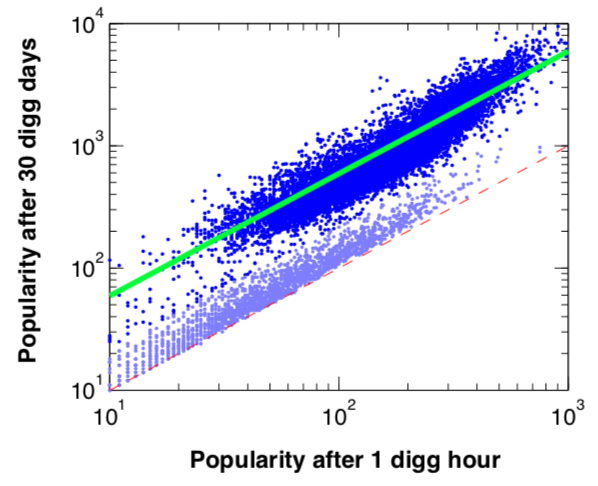
\includegraphics[width=\textwidth]{digger}
      \caption{}
      \label{}
    \end{subfigure}%
    ~%add desired spacing
    \begin{subfigure}[b]{0.5\textwidth}
      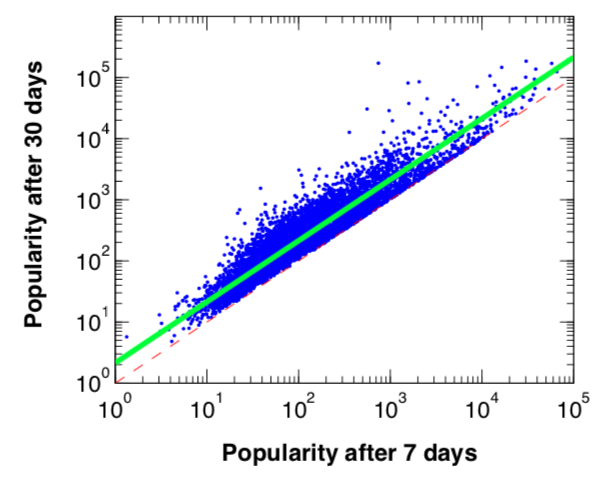
\includegraphics[width=\textwidth]{youtube}
      \caption{}
      \label{}
    \end{subfigure}
    \bicaption{消息流行度展示。(a)Digg 数据集,(b)Youtube 数据集。\citep{szabo2010predicting}}{Message popularity display. (a)Digg data, (b) Youtube data.\citep{szabo2010predicting}}
    \label{fig:digger-youtube} 
\end{figure}

Lee 等 \citep{Lee2010An}认为在线文本的流行度有时本身就不能被预测,所以没有预测 在线文本的流行度而是利用比例风险回归模型对文本早期信息的特征进行研究,预测其是否会流行。Jamali 等 \citep{Jamali2009Digging}使用 Digg 信息的评论数量、评论的平均字数 和评论树状结构作为特征,训练他们的回归模型。Tatar 等 \citep{Tatar2011Predicting}用信息在其发布 的一段时间后获得的评论数作为因子,提出了一个简单有效的线性回归模型,预 测其后期的流行度。Bao 等人 \citep{Bao2013Popularity,Gao2014Popularity}研究了以微博消息为研究对象,研究了消 息流行度预测与消息早期传播的网络结构之间的关联性,如图\ref{fig:str}所示,消息未 来的流行度与消息早期传播的链接密度存在很强的负相关性,和消息早期的传 播深度存在近似的线性相关性。于是,基于初始阶段用户之间链接密度和微博的 传播深度,分别提出了两个微博流行度的预测模型。第一个模型是在微博转发 的初始阶段,基于微博的转发深度来预测微博的转发量;第二个模型是在微博 转发的初始阶段,基于用户的链接密度来预测微博的转发量。Cheng 等 \citep{Cheng2008An}采用 了时间序列模型中常用的自回归移动平均模型 (Autoregressive Integrated Moving Average Model,ARIMA),对网络上跟帖数量随时间变化的趋势情况进行了预测 分析。

 
 \begin{figure}[H]
    \centering
    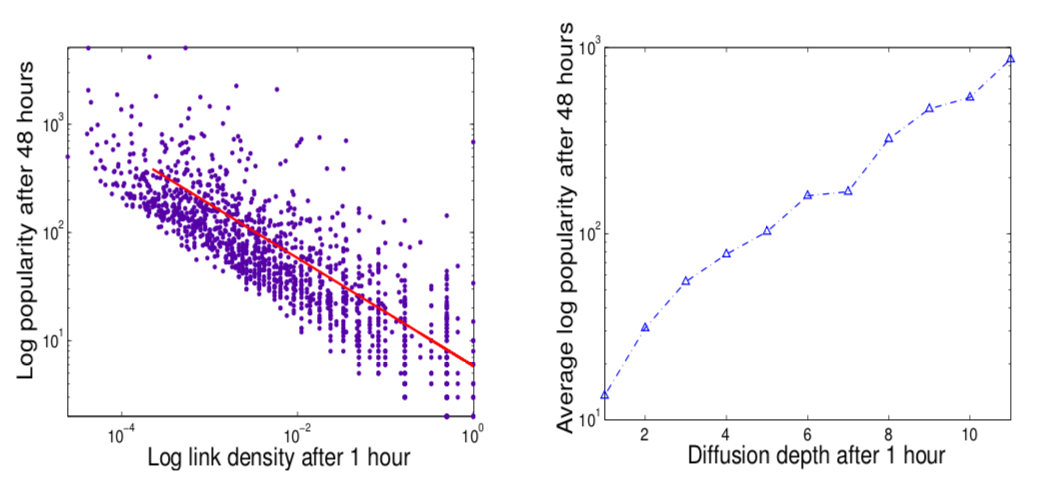
\includegraphics[width=0.5\textwidth]{str}
    \bicaption{结构特性\citep{Bao2013Popularity}}{Structural characteristics\citep{Bao2013Popularity}}
    \label{fig:str}
\end{figure}

\subsection{基于时间序列的方法}
基于时间序列建模的预测方法主要关注用户传播过程对应的时间序列。这 类方法在对时间序列建模后,利用所得的模型进行用户生成内容的流行度预测 工作。Yang 等 \citep{Yang2011Patterns} 研究了用户生成内容流行度随时间的消涨模式。该研究利 用 K-谱中心聚类算法和逻辑回归模型,通过对 5.8 亿条推文和 1.7 亿篇博客文 章流行度随时间消涨模式的聚类分析,挖掘出 6 类形态各异的流行度时序模式。 Matsubara 等 \citep{Matsubara2012Rise}做了进一步研究,用 SpikeM 模型对上述 6 种时序模式进行拟 合,利用 SpikeM 模型进行流行度预测。SpikeM 模型利用幂律分布描述用户生成 内容的传播能力随时间衰减的过程,并利用正弦方程描述用户关注度随时间周 期变化的过程。Figueiredo 等 \citep{Figueiredo2014TrendLearner}利用极随机集成树将时间序列分类,从而预测 信息的趋势。Hu 等 \citep{Hu2016Predicting}通过对短期爆发的热门话题流行度时间序列进行分析,发现这些序列具有高度相似性,进而定义流行度时序特征空间,即流行度的平均 值、走势和周期,以分析流行度随时间的变化趋势。

\subsection{基于传播模型的方法}

传播模型最早是流行病学中对病毒扩散机制的研究,社交网络中的消息传播机制可以和病毒在人群中的传播方式进行类比。两者的不同之处在于,社交 网络是存在一定的网络结构的,消息一般是沿着社交网络结构进行扩散。并且, 用户之间的消息传播概率和病毒传播的概率也有较大区别。传播过程分析和动 力学研究是预测信息流行度的重要基础。以生物数学领域中的流行病模型为基 础,构建新的传播规则和模型是微博流行度预测的一种重要方法。这些模型通 常把微博网络中的用户节点划分为未知者、传播者和免疫者三大类。在消息传 播网络中,给定一条微博消息,未知者表示从没有接触过该消息的用户,传播者 表示接触过该消息并且以一定概率传播该消息的用户,免疫者表示了解消息但 不会进行传播的用户。在消息传播过程中,传播行为主要发生在不同状态节点 相互连接所产生的边。在 Daley 等人 \citep{Daley1965Stochastic}提出的 DK 模型中,若传播者遇到未 知者,未知者则以一定的概率变为传播者;若传播行为发生在 2 个传播者之间 时,两者都会以一定概率转化为免疫者。Maki 等人 \citep{Maki1973Mathematical} 提出的 MK 模型的传播 规则有所不同,即当 2 个传播者相遇时,只有一个传播者以一定概率变为免疫 者。Xiong 等人 \citep{Xiong2012An}将用户分为易感染人群、接触信息人群、感染人群和康复人 群类,建立了基于转发机制的信息传播模型。研究结果发现,无标度网络中的接 触信息人群比规则网格中的多;感染者的密度随着点度的增加而增长。Wang 等 人\citep{WANG2013ReTweeting} 发现微博传播与 SIS(susceptible-infectious-susceptible) 模型存在许多相似 性,因而利用 SIS 模型预测微博转发行为,实验结果显示,预测的错误率很低。 Yang 等人\citep{Yang2011Modeling} 在 SIS 模型的基础上提出了线性影响模型,根据当前微博信息的 流行度预测未来某一时间的流行度。模型假设微博信息的传播受各节点影响力 支配,为每个节点建立影响函数以量化该节点对后续被激活节点的影响力,从而 把流行度预测转换为活跃节点的影响力计算问题。


基于传播模型的方法还有一种是将在线内容的受欢迎度累积为转发过程,并 对每个消息的到达过程中的强度函数进行独立的建模。Shen 等 ­\citep{Shen2014Modeling} 采用了强化 泊松过程 (Reinforced Poissopn Process,RPP) 来对社交网络中的三种现象进行建 模: 一个消息的固有吸引力,对吸引力的短暂放松,以及富者愈富的机制,公 式如\ref{eq:xd}所示,$i_d(t)$就是富者愈富的影响,其概率图表示如图\ref{fig:c}所示。


\begin{equation}\label{eq:xd}
\lambda_d(t) = \lambda_d f_d(t,\theta_d)i_d(t)
\end{equation}



其中,$\lambda_d$为消息的固有吸引力,时间松弛函数 (temporal relaxation function)  $f_d(t,\theta_d)$刻画了吸引力时效性对消息传播速率的影响,$\theta_d$为松弛函数的参数,$i_d(t)$
表示消息 \textit{d} 在时刻 \textit(t) 已经收到的关注数。该模型在论文引用网络中进行了验证, 其中,时间松弛函数如公式\ref{eq:fd}, 反映了论文影响力的时间衰减效应。此处,自增 强采用的是线性函数,反映了论文吸引力随着引用次数的增加呈线性增长。

\begin{equation}\label{eq:fd}
f_d(t) = \frac{1}{\sqrt{2\pi}  \sigma_dt}\exp(-\frac{(\ln t - \mu_d )^2}{2\sigma_d^2})
\end{equation}

\begin{figure}[H]
    \centering
    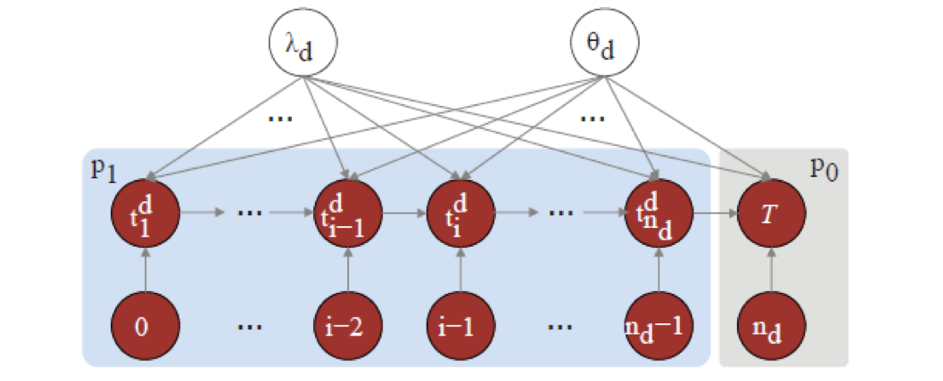
\includegraphics[width=0.5\textwidth]{c}
    \bicaption{RPP概率图\citep{Shen2014Modeling}}{RPP probability graphical\citep{Shen2014Modeling}}
    \label{fig:c}
\end{figure}


Gao 等人\citep{Gao2016Modeling}在研究中发现消息传播中关键用户的影响,提出了混合的 RPP 模型,将消息的传播看成是多个由关键用户节点引起的 RPP 子过程的混合,如 图\ref{fig:d}所示。将 RPP 模型扩展到不同的时间松弛函数,并将其应用于动态转发过 程的预测。后来,利用 RPP 模型中的转发数量,来模拟富者愈富的现象,利用 Hawkes 自激励点过程直接对每个消息转发的具体贡献进行建模,其特征为用户 影响和时间松弛函数。Hawkes 过程为我们提供了一个通用的框架来建模一个信 息如何引起注意的过程,这使我们非常容易理解信息级联的底层机制。此外,还 采用深度学习技术来学习到达率在点过程中的作用。无论如何,这些方法通常 不会对未来的流行度进行直接优化,并且这些方法是独立地为每个消息学习参 数,缺乏实际应用能力。因此,他们不能充分利用流行度预测中的隐含的级联 信息, 在可解释性和可预测性之间仍然存在差距。为了解决这一难题,通过学习 Hawkes 过程的内部因素,即: 在端到端监督框架下,用户影响、自激励和时间衰 减等不同的因素的影响,为流行度预测的可解释性和可预测性提供更好地解决 方案。

\begin{figure}[!htbp]
    \centering
    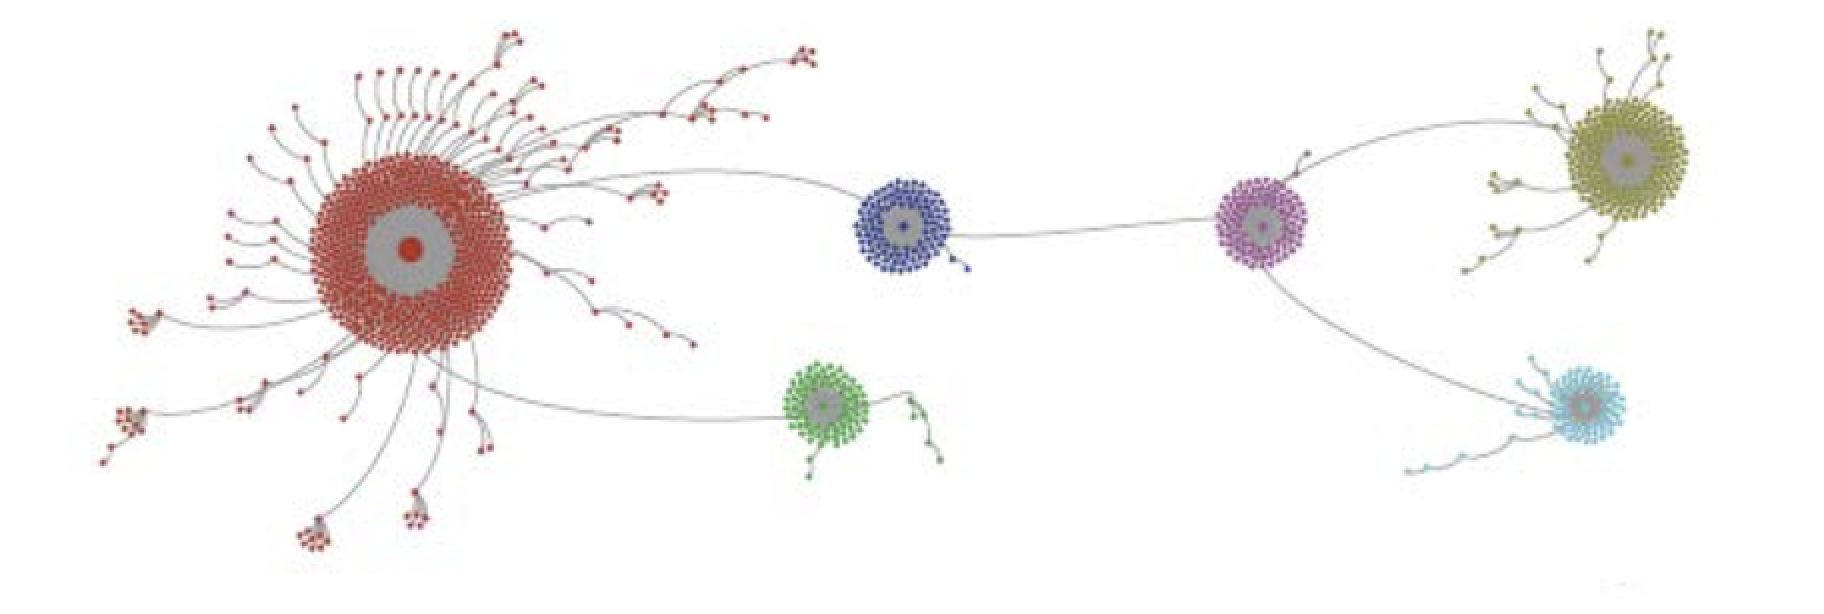
\includegraphics[width=0.7\textwidth]{d}
    \bicaption{新浪微博中某消息的传播拓扑结构图\citep{Gao2016Modeling}}{A Topology Of The Spread Of A Message On Sina Weibo\citep{Gao2016Modeling}}
    \label{fig:d}
\end{figure}

\section{深度学习背景}
近年来,深度学习作为一个强大的工具在多个领域取得了成功的应用,在社 交网络领域,也有不少相关的尝试,均取得了不错的效果,说明了深度学习模型 在社交网络分析领域有巨大的运用价值。在消息传播预测中,消息的传播过程就 是一个明显的序列过程,将消息在用户之间的互相传播过程解析成一系列的序 列过程,在这个过程中,应用深度学习中的循环神经网络处理是十分方便的,因 此深度学习在消息预测中有着十分广阔的应用。
\subsection{深度学习简介}
深度学习是利用一个层次化的架构学习出原始输入在不同层次上的表达,在 这个层次化中,高层的概念通常是通过低层的概念来定义的,这种层次化的表达 可以帮助解决更加复杂抽象的任务。深度学习通常使用人工神经网络,常见的具 有多个隐层的深度神经网络 (DNN) 就是典型的深度架构。很多深度学习模型有 其仿生学基础,因为人的信息处理系统是清晰的层次化的结构,比如人类的听觉 系统以及视觉系统,所以很自然地,人们相信如果能够构造类似的深度架构和相 应的学习算法会对处理这种类型的自然信号有很大的帮助。此外,从理论角度, 这种层次化的结构在表达某些特定运算的时候往往能够比浅层架构更加高效。

深度学习一直面临着计算量大、难以优化以及容易过拟合等问题。转机出现 在 2006 年,一直致力于神经网络以及深度学习研究的 Hinton 等人使用无监督的 逐层处理的预训练方法成功减轻了深度模型学习困难的问题,从而掀起了深度 学习的浪潮 \citep{Sch2006Efficient}。近年来,随着计算能力的不断提升、数据量的不断增加以及新 的训练方法的提出 \citep{Srivastava2014Dropout},深度学习得到进一步发展,深度模型的效果也越来越明 显,最终在语音识别、自然语言处理和图像处理等一系列难题上取得了巨大的突 破,并得到了学术界和工业界的广泛重视。在语音领域,从 2009 年开始,微软 研究院和 Hinton 合作率先在语音处理中使用深度神经网络,从而使得语音识别成为深度学习取得突破的第一个领域 \citep{Hinton2012Deep,Deng2013New}。在图像领域,2012 年,Hinton 团 队的 Krizhevsky 等人 \citep{Krizhevsky2012ImageNet}  使用深层次的卷积神经网络在 ImageNet 评测上取得巨 大突破,将错误率从 26\% 降低到 15\%,重要的是,这个模型中并没有任何手工 构造特征的过程,网络的输入就是图像的原始像素值。在此之后,采用类似的架 构,通过使用更深更复杂的模型、更多的参数以及训练数据,ImageNet 评测的 结果得到进一步大幅改善。这期间典型的模型包括 Google 构建的 24 层的深度神 经网络 GoogLeNet\citep{Szegedy2015Going}以及微软构建的 152 层的深度网络  \citep{He2016Deep,He2016Identity} 等。

\subsection{循环神经网络概述}

循环神经网络(recurrent neural network,RNN)是上世纪 80 年代末提出的 一种针对处理时间序列输入的神经网络。循环神经网络相对于传统的前馈神经 网络主要具有以下特点:(1) 前馈神经网络的网络拓扑结构构成了一个有向无环 图,信息沿着一个方向从输入节点传递到输出节点。循环神经是一种带环的神 经网络,网络中产生的信息会反馈到后面的计算中。(2) 前馈神经网络主要处理 静态的输入输出数据,而循环神经网络主要用来模拟动态系统或者建模变长序 列数据。RNN 的这种环状连接在网络内部构成一种用来刻画动态变化的状态信 息。RNN 可以用这种内部状态存储机制来处理任意的序列输入。因此 RNN 适用 于很多序列相关的应用,比如语音识别、自然语言理解等。(3) 循环神经网络可 以按照序列顺序,展开得到一个前馈神经网络的形式,但是由于 RNN 每一步计 算中采用同样的函数,因此,循环神经网络可以认为是一种在所有层之间共享参 数的前馈神经网络。基础的 RNN 的计算公式如\ref{eq:2-rnn}所示, 其中,$h_t$为 t 时刻的表 达,$x_t$ 为 t 时刻的输入,W,U,b 是模型的参数。

\begin{equation}\label{eq:2-rnn}
h_t = g(Wx_t + Uh_{t-1} + b)
\end{equation}

前馈神经网络主要基于反向传播进行梯度求解 \citep{Rumelhart1988Learning,Werbos1994The}。由于循环神经网络 可以认为是共享参数的前馈神经网络,因此主要采用时序反向传播算法。这种算 法是传统反向传播算法的一种扩展。我们先将一个循环神经网络展开成共享参 数的前馈神经网络,然后,基于这个前馈神经网络进行后向传播。最后,把每一 层中相应的参数梯度相加,则得到该共享参数的梯度。有时候展开得到的前馈神 经网络可能太长,因此常用的训练方法还有截断的时序后向传播算法。
\subsection{基于表示学习的方法}
由于社交网络的开放性和复杂性,网络内容的流行度预测是十分困难的。影响网络内容的未来流行程度有各种各样的因素。为了处理这种复杂的流行动态, 并从原始数据中自动提取有用的信息,基于表示学习的方法正在应用到流行度 预测中。Mishra 等人 \citep{Mishra2016Feature}提出了一种两阶段模型,将 Hawkes 点过程的参数作 为表示,并将其与其他提取的特征结合到机器学习模型中,来进行流行度预测。 Hoang 等人\citep{Hoang2017GPOP}提出将用户分组形成聚簇,然后采用张量分解进行预测。这个 方法实际上是学习在空间中每个消息的表示形式,它是由与用户组相对应的维 度来表示的。深度学习的成功,也激发了对级联预测的端到端表示学习框架。Li 等人\citep{Li2016DeepCas}提出了 DeepCas,其模型结构如图\ref{fig:deepcas}所示,它通过随机游走将级联图 作为节点序列,并在深度学习框架下学习每个级联的表示。

\begin{figure}[!htbp]
    \centering
    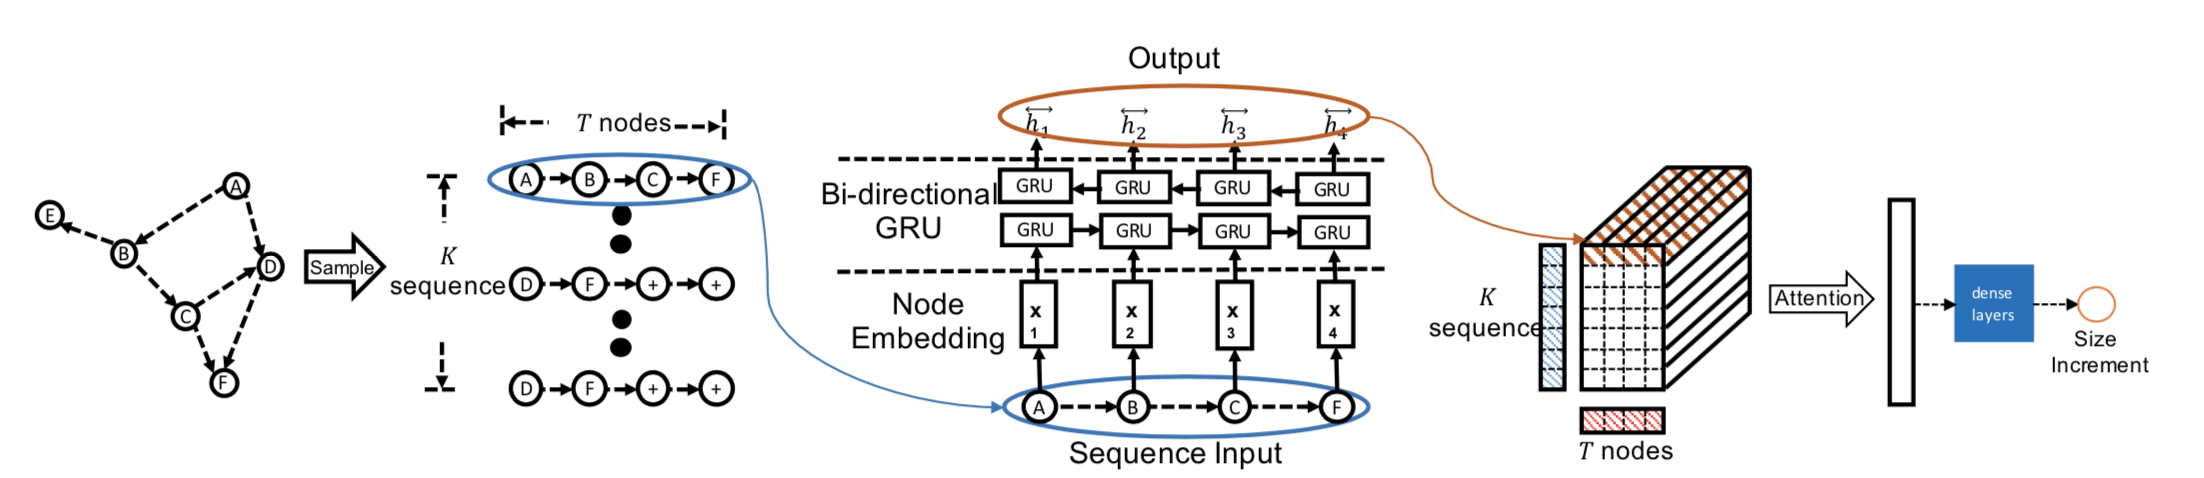
\includegraphics[width=1\textwidth]{deepcas}
    \bicaption{DeepCas模型\citep{Li2016DeepCas}}{DeepCas model\citep{Li2016DeepCas}}
    \label{fig:deepcas}
\end{figure}


表示学习的一系列的工作可以自动地从数据中学习有价值的表示,并成功 应用到其他领域的表示学习中。然而,现有的研究要么采用了两阶段的方式 \citep{Mishra2016Feature}, 缺乏作为表征学习的指南,要么忽略了传统研究所揭示的预测信息,例如,Deep- Cas\citep{Li2016DeepCas} 忽略了影响流行度预测的时间特征。此外,深度学习方法缺乏清晰的解 释性来帮助我们理解信息级联的流行动态的内在机制。在 Cao 等人\citep{Cao2017DeepHawkes}提出的 DeepHawkes 模型中,在深度学习的框架下,使用端到端的方式,直接建模未来 流行度。该方法刻画了已有的 Hawkes 模型中的信息传播过程中比较关键的因子 或机制,对未来流行度预测有很好的参考价值,其模型如图\ref{fig:f}所示。

\begin{figure}[H]
    \centering
    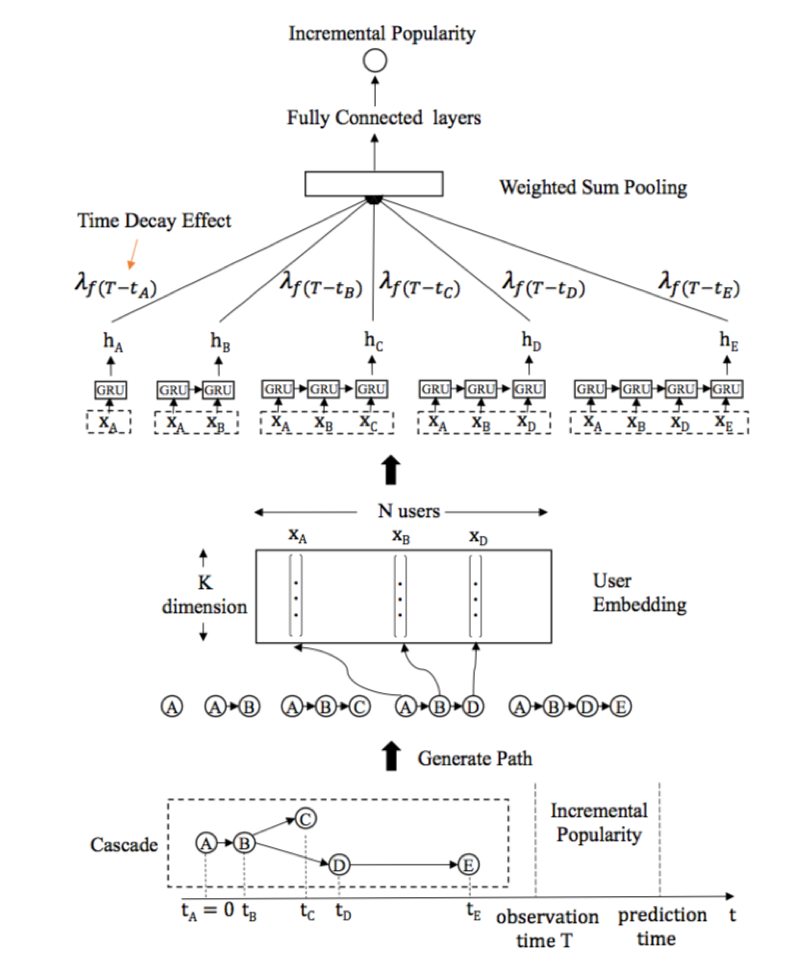
\includegraphics[width=0.5\textwidth]{f}
    \bicaption{DeepHawkes模型\citep{Cao2017DeepHawkes}}{DeepHawkes Model\citep{Cao2017DeepHawkes}}
    \label{fig:f}
\end{figure}

在社交网络消息转发预测方面,Zhang 等人 \citep{Zhang2016Retweet}主要是针对 Twitter 上消息 的转发问题进行了研究,将其建模成二分类问题,给定用户和消息,预测用户是 否会转发该消息。通过神经网络学习消息的内容表达,通过注意力机制学习用户 的兴趣表达,网络结构如图\ref{fig:dnn-attention}所示。该模型利用用户的历史发布消息学习用户 的兴趣表达,通过神经网络将转发消息有机结合起来,提高了模型的预测效果, 但是该方法与 Du 等人 \citep{Du2016Recurrent}的研究工作相比,没有考虑到消息传播中的时间序列 特征,而该特征在很多研究中已经证明了其重要性,因此该方法还有很多改进的 空间。

\begin{figure}[H]
    \centering
    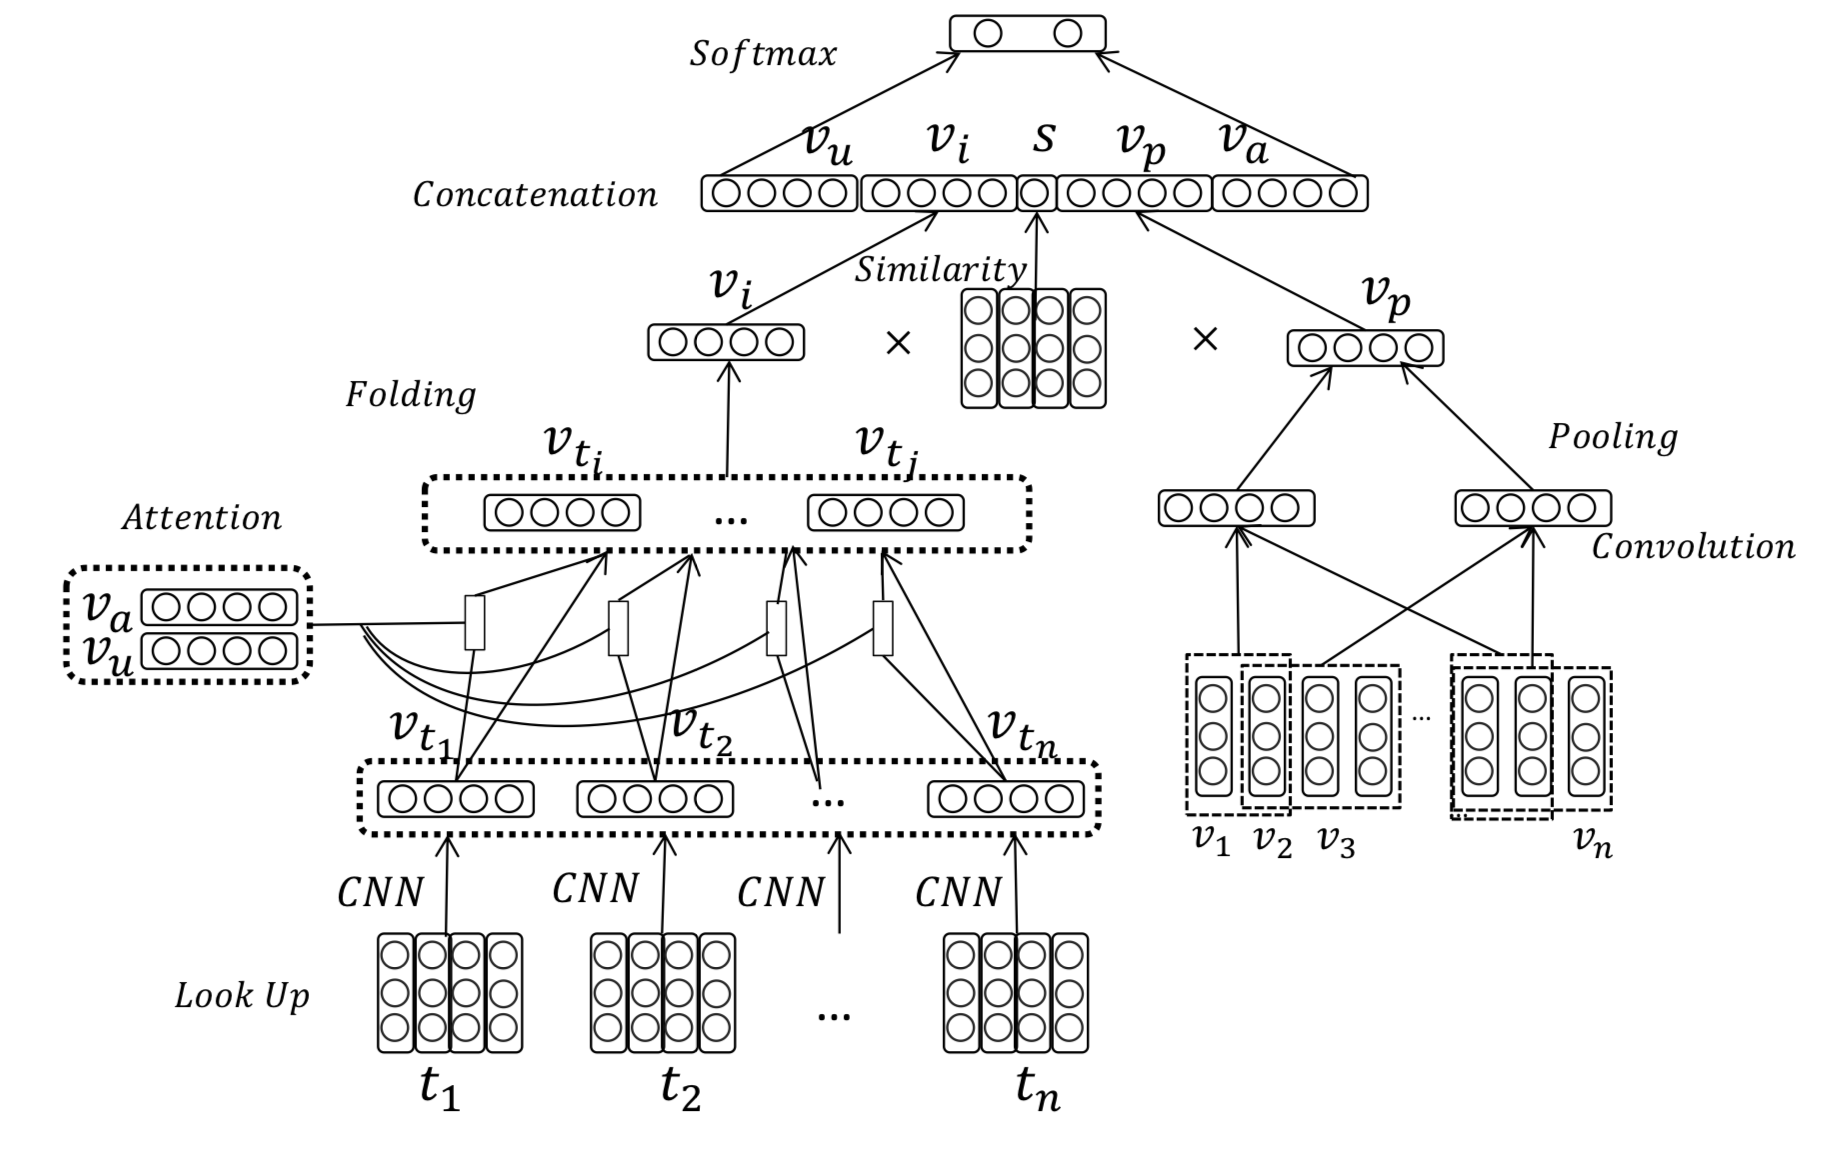
\includegraphics[width=0.8\textwidth]{dnn-retweet}
    \bicaption{基于注意力机制的预测模型\citep{Zhang2016Retweet}}{Predictive model based on attention mechanism\citep{Zhang2016Retweet}}
    \label{fig:dnn-attention}
\end{figure}

\section{Hashtag流行度预测的方法}

Hashtag 的流行度预测主要是指 Hashtag 在一段时间内被使用的情况, 这种情 况主要通过 Hashtag 的使用频次界定。Kong 等人 \citep{Kong2014Predicting}根据 Hashtag 生命周期中 的使用频次的变化情况定义了 Hashtag 的 4 种流行度类别: 出现、爆发、平静、沉 寂,Ma 等 \citep{Ma2012Will,Ma2013On} 也按照 Hashtag 的使用频率划分 Hashtag 的流行度。通过对流行 度的类别划分可以将 Hashtag 的流行度预测问题转化为分类问题, 按照不同的频 次等级对 Hashtag 进行类别划分, 使用分类器对 Hashtag 进行流行度类别的预测, 从而预测 Hashtag 在未来的使用频次,Hashtag 的分布也是呈现幂率分布的,如 图\ref{fig:g}所示。

\begin{figure}[H]
    \centering
    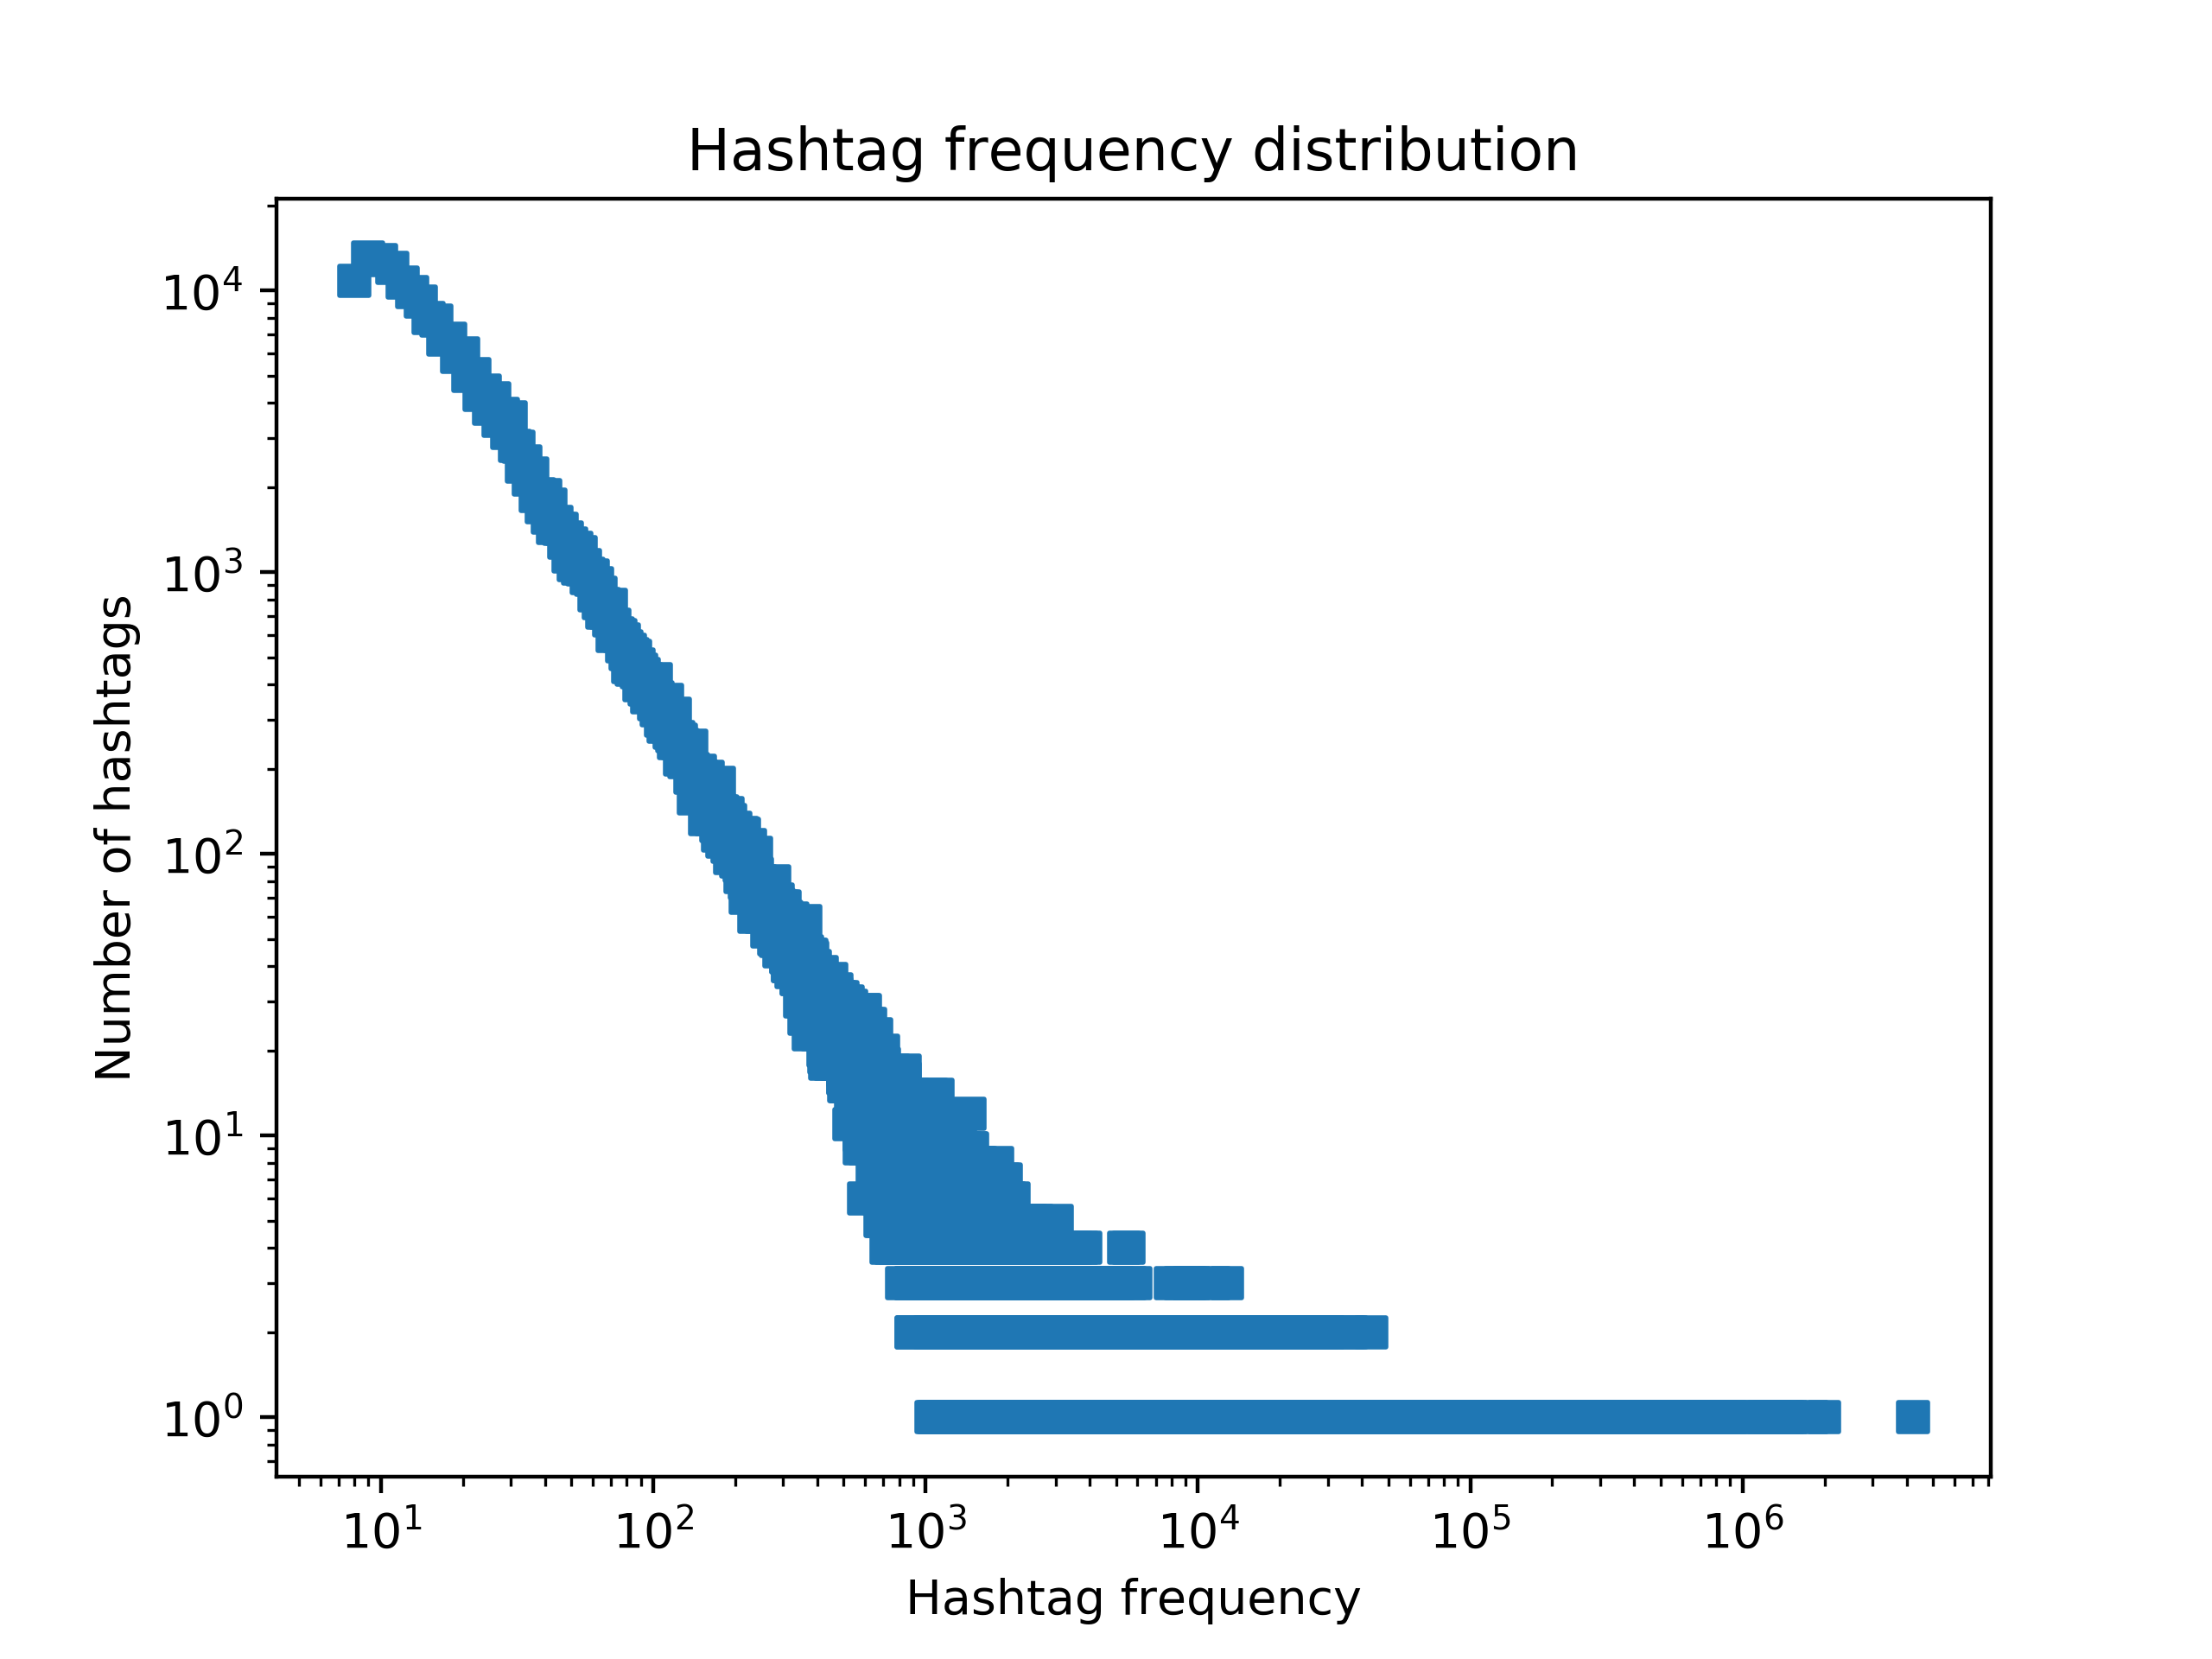
\includegraphics[width=0.5\textwidth]{hashtag_5}
    \bicaption{Hashtag频率分布}{Hashtag Frequency Distribution}
    \label{fig:g}
\end{figure}


目前 Hashtag 流行度预测的方法主要集中在研究其特有特征以及微博消息 的不同类型的特征,根据其不同特征,进行机器学习模型的优化。例如在前期的 研究中,Zongyang Ma 等人\citep{Ma2013On}在判断一个 Hashtag 是否会流行,考虑了内容特 征以及上下文特征,具体特征如表\ref{tab:hashtag-feature}所示。Oren Tsur 等人 \citep{tsur2012s}在预测 Hashtag 的流行度时,考虑了四中主要特征,包括 Hashtag 的内容,全局特征,图特征, 以及时间序列特征,论证了不同特征在模型中的重要性。但是目前的基于特征的 方法没有分析用户粉丝之间的网络结构特征以及对于 Hashtag 自身的特性挖掘 较少,模型的效果还有很大提升空间;另一方面,在刻画 Hashtag 主题标签内部 传播机制方面还没有研究,并且 Hashtag 是多源头的,不同的用户可以在不同的 时刻不断产生和转发,不同于传统的单源头消息预测,因此如何刻画多源头的主 题标签传播机制是一个研究的方向。

\begin{table}[!htbp]

    \bicaption{Hashtag特征}{Hashtag Feature}
    \label{tab:hashtag-feature}
    \centering
    \footnotesize% fontsize
    \setlength{\tabcolsep}{4pt}% column separation
    \renewcommand{\arraystretch}{1.2}%row space 
    \begin{tabular}{|l|l|}
        \hline
        \textbf{Type} & \textbf{Description}\\
        %\cline{2-9}% partial hline from column i to column j
        \hline
        \multirow{6}{*}{\textbf{Content Feature}}& number of tweets in Tth\\
&fraction of tweets containing URL\\
&fraction of retweet\\
&fraction of tweets with mention"@"\\
&hashtag clarity\\
&20-dimension hashtag topic vector\\ \hline

\multirow{8}{*}{\textbf{Context Feature}}
&number of users |Uth|\\
&average authority of users\\
&density of Gth\\
&fraction of users forming triangles in Gth\\
&ratio between the number of connected components and the number of nodes in Gth\\
&average edge weights in Gth\\
&number of border users\\
&15-dimension exposure probability vector\\ \hline
    \end{tabular}
\end{table}

\section{本章小结}
本章对传统消息流行度预测的方法以及 Hashtag 的流行度预测方法的相关研究工作进行了总结,并介绍了消息表示学习的研究进展,为后文基于用户粉丝网络结构特征的主题标签流行度预测算法和基于深度神经网络的多源头主题标 签流行度预测方法提供了理论基础。在传统的消息流行度预测方法上,主要还是 采用机器学习的方法,深度挖掘消息传播过程中的有效特征,该方法在实际应用 中效果较好,但是没有考虑 Hashtag 自身的情感性、地域性和事件性等特征以及 用户网络结构特征,因此本文在此方面考虑 Hashtag 的自身特性以及用户网络结 构特征,提出新的有效特征。另一方面目前深度学习在很多方面有了成功应用, 并且在消息预测上有了初步尝试,为后续多源头主题标签流行度预测提供了新 的思路。